% Pursuing Stacks (cotes 134-2 to 134-8): archive cote 134-4, site page 43 (PDF page 44), typescript page 131.
% typescript. Draft compared: ps3.tex:2168-2238.
% AI-transcribed by Claude Opus 5.5 (claude-opus-5-5, adaptive thinking, effort high), Message Batches API, batch ps2 (msgbatch_01NVwr1Yuo8qJf5rykeGBXPK), 2026-11-12; image review recorded in records/CHECK_DECISIONS_134_3_4.tsv.
\scanpage{134-4/43}
\mspage{131}

We'll say the functor u is \uline{compatible with the homotopy structure} h
on M, if it satisfies the equivalent conditions (i),(ii), i.e. if it
factors as in (1) above. In case u commutes with finite products, and
if either the homotopy structure h can be described in terms of weak homo-%
topy intervals, or in terms of contractible objects, the compatibility
of u with h can be checked correspondingly, either by (i'), or by (ii').

\margin{54.} An important particular case is the one when
\[ N = W^{-1}M \]
is a localisation of N by a \xout{\unsure{sub}}set of arrows in M
\[ W \hand{\subset} F\over{l}{\ell}(M) \ . \]
We'll say that the homotopy structure h on M is \uline{compatible with} W , if
\inserted[typed]{it is with} the canonical functor $M \hand{\to} W^{-1}M$ . If W is \uline{strongly saturated}, this
is most readily expressed by the condition that $W_h \hand{\subset} W$ i.e. any homotopi\hand{\unsure{sm}}
is in W ( i.e. \xout{is} "any homotopism is a weak equivalence", if the elements
of W are named"weak equivalences"); in case M admits finite products and
the localization functor commutes to these (e.g. the case (M,W) is a
\uline{strict} modelizer), \xout{this also means that the for} and if moreover \over{\unsure{h}}{h} is a
contractibility structure, \xout{this also} is is sufficient to check that
for any contractible X, the projection $X \hand{\to} E$ is in W. \diagram{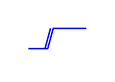
\begin{tikzpicture}[baseline=-.4ex,x=1em,y=1ex]\draw[color=blue,line width=.5pt] (0,0)--(.7,0)--(.9,1.7)--(2.1,1.7);\draw[color=blue,line width=.5pt] (.6,0)--(.8,1.7);\end{tikzpicture}}If we dont assume
or know beforehand that W is strongly saturated, but just saturated say,
we may still introduce a more stringent compatibility condition, by
saying that \xout{the} the homotopy structure h and W are \uline{strictly compatible}
if $W_h \hand{\subset} W$ . Using the \xout{strict} saturation condition c') on W, it is easily
seen that in the case \deleted{above} when h is a contractibility structure, \deleted{and}
\deleted{the functor $M \ W^{-1}M$ commutes to finite products,} then \deleted{it is enough to} \inserted{$W_h \subset W$ \deleted{\illegible{1}} (strict compa-%
tibility) is equivalent to: for}
\deleted{check that for} contractible X, the projection $X \hand{\to} e$ is \xout{in W. \illegible{1}} \inserted[typed]{"universally in W"}\hand{,}
\inserted[typed]{or (as we'll say) W-\uline{aspheric}.}
Indeed, to deduce from this that any homotopism $f: X \hand{\to} Y$ is in W, we
are reduced to checking that any endomorphism of either X or Y which is
homotopic to the identity map, is in W. Now this will follow from the
assumption, and the following

\uline{Proposition} Assume the homotopy structure h on M can be defined by a
generating set $\hand{\Sigma}_h^o$ of weak homotopy intervals $\underline{I} =(I,\hand{\delta}_o,\hand{\delta}_1)$ which are
W-\uline{aspheric} (i.e. I W-aspheric over \inserted{e}\xout{\unsure{I}\illegible{1}} ), \over{t}{w}\over{h}{h}ere W \xout{is}$\hand{\subset} F\over{l}{\ell}(M)$ is \inserted{any} saturated \inserted{subset}
(in fact, mildly saturated is enough). T$\overset{\hand{\scriptscriptstyle\perp\perp}}{\mathrm h}$en W is the inverse image \xout{of}
by the canonical functor $M \hand{\to} M_h = \overline{M}$ of a \xout{mildly} subset $\overline{W} \hand{\subset} F\over{l}{\ell}(\overline{M})$, i.e.
\xout{the relation} if f,g are homotopic arrows in M, if one is in W, so is the
other. Moreover (if W is saturated) $W_h \hand{\subset} W$ i.e. h and W are \over{st}{st}rictly
compatible.

\margin{43}
